\chapter{Introduction}
\begin{figure}[h]
\centering
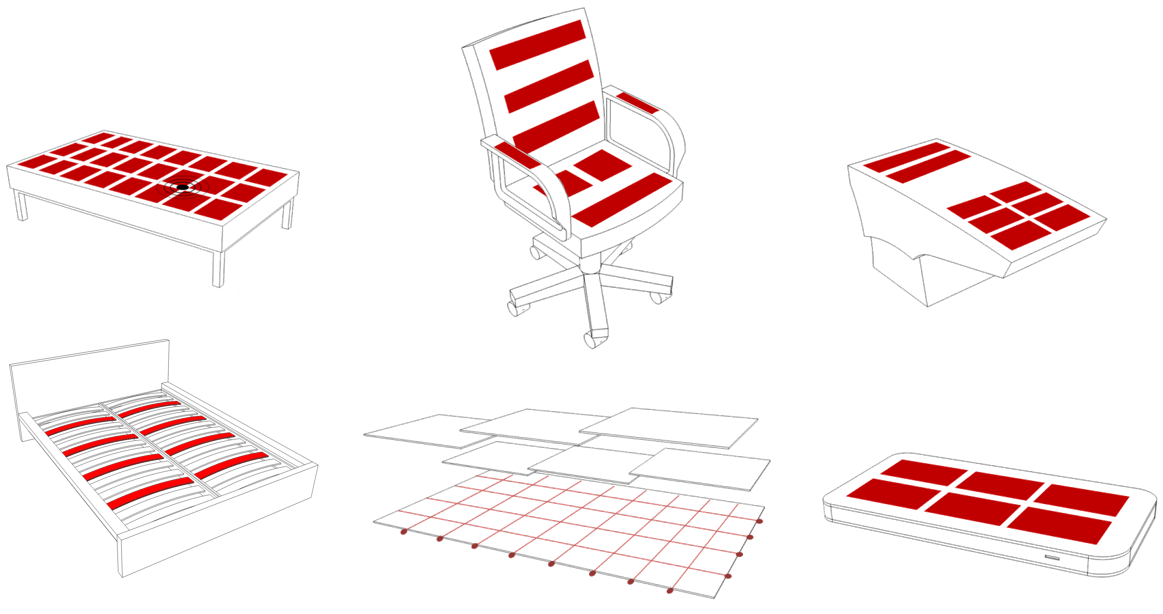
\includegraphics[width=0.9\textwidth]{images/all_protos}
\caption{Sketch of electrode placement of all capacitive sensing prototypes created in the scope of this work}
\label{fig:all_protos}
\end{figure}
Smart environments are comprised of numerous sensing and computing devices that are supporting a number of users in this environment on performing their tasks. Driven by advances in computing power, miniaturization of sensors and processing methods, novel devices including a plethora of functionality have been introduced into our everyday lives.  In science the field has been thriving in the last decades, combining knowledge from disciplines including computer science, engineering, but also product design, in order to create systems that are integrated into the environment, have a high usability and provide information and services to the actors in smart environments. Perhaps the most cited example of this trend is the rise of the smartphone, from professional business tool to a consumer device being sold hundreds of millions times a year. Using integrated sensors and communication facilities it is possible to provide services aware of location, schedule, contacts, or preferences, that realize navigation, event planning, augmented reality, or entertainment. A different example are increasingly networked homes that are aware of energy usage, lighting levels, temperature and the status of critical devices and can be controlled by the user from a single place or autonomously using a set of specified rules. 

A common aspect of all smart environments and smart devices is sensing. This includes environmental parameters but also system state and most importantly the activities of the different users. There are numerous categories of sensing devices that can realize different aspects of this sensing, ranging from cameras or accelerometers to GPS and acoustic sensors. Capacitive sensors are a category of sensors that use electric fields to sense the presence and certain properties of the human body. The most common variety is sensing the presence of fingers on touch screens, already present in billions of devices. However, there is another variety, the capacitive proximity sensor that is able to detect the presence of human body parts over a distance, providing interesting applications in smart environments, by unobtrusively integrating the sensors into different materials, environments and appliances. When designing an application of smart environments choosing the right sensors is one of the most relevant decisions that has to be taken early in the process. Even though there are numerous prototypes available, so far this process has been mostly supported by looking at previous activities. 

In this work I present a benchmarking model that can support this decision process in the domain of smart environments, in order to determine relevant application areas for capacitive proximity sensors. There are numerous challenges associated to each area, regarding the details of the application. I will present a collection of existing and novel methods that support processing data generated by capacitive proximity sensors. Several prototypes created using those methods have been implemented and evaluated for performance and usability. Figure \ref{fig:all_protos} shows sketches of the different prototypes and the placement of the electrodes attached to the capacitive proximity sensors. Based on this evaluation and the knowledge generated in the design process I am able to discuss the benefits and limitations of the technology, classify it with regards to competing technology, in order to present a set of guidelines that can aid parties interested in designing smart environment applications using capacitive proximity sensors.
 
\section{Motivation}
In the last decade the way we interact with computing machines has changed in a profound fashion. Today more than one billion people operate a smartphone, enabling ubiquitous access to communication tools, processing power and information. The vision of ubiquitous computing as proposed by Mark Weiser in the early 90s is inching closer to reality \cite{Weiser1991}. The required technologies of \begin{quote}
"cheap, low-power computers that include equally convenient displays, a network that ties them all together, and software systems implementing ubiquitous applications" 
\end{quote}
are now existing in the form of smartphones and tablets that are connected to the internet, using high-speed connections such as LTE and web-based services such as Google Now, that combine numerous data sources to provide personalized services.

While the vision and underlying ideas remain similar other names have been used in research, including Pervasive Computing and Ambient Intelligence. The concept has been expanded to not only consider devices that can be directly manipulated, but include determining the situation and reacting based on it. This context-aware computing proposes 
\begin{quote}
"systems that examine and react to an individual's changing context. Such systems can promote and mediate people's interactions with devices, computers, and other people" \cite{schilit1994context} 
\end{quote}
Different forms of context can be distinguished, ranging from location and the actual system state, to different activities or even the current mood of the user. In order to acquire this context, the input-and-output based systems originally proposed by Weiser, are augmented by an ensemble of devices that are very small (dust), coordinate in massive numbers (clay) or are flexible, unobtrusive extensions to everyday objects (fabric) \cite{poslad2011ubiquitous}. This devices can be invisibly integrated into our everyday environment and provide sensing capabilities that can be used by sufficiently smart systems. Examples of these devices are microelectromechanical systems (MEMS) or bendable technology, such as OLED screens. The number of computation and sensing devices that we carry with us is growing continuously, yet we want the technology to further disappear, allowing us to focus on the application instead of the underlying technology. 

The famous science fiction author Arthur C. Clarke proposed three laws of prediction, the  third of which is 
\begin{quote}
"Any sufficiently advanced technology is indistinguishable from magic." \cite{clarke1962hazards} 
\end{quote}
Capacitive proximity sensing allows us to measure the influence of the human body (or conductive objects in general) on an electric field. While we would not call this technology magic, a peculiarity of electricity is that humans have no specific sensing organs, thus we generally remain unaware of their presence, unless the field strength is very high. Consequently, when interacting with capacitive sensors there is no awareness of what they are sensing unless it is specifically exposed to the user. The technology is well-understood and varieties have become ubiquitous in some areas, such as touch screens. However, there are numerous other applications for this technology, ranging from industrial fluid level and material detection, to presence detection for cars. A particularly interesting domain for this sensing technology are smart environments that provide services based on unobtrusively acquired information about persons currently acting in this environment. There are numerous sensing technologies that provide similar detection capabilities. Looking at the recognition of simple activities, such as standing, walking and lying, cameras and accelerometers can lead to the same result. Accordingly, in order to discuss the use a sensing technology within a specific domain, it is necessary to provide a benchmark that takes into account abstracted sensor properties and different application domains. In this work we will provide a generic benchmark model for different sensor technologies in smart environments and based on this discuss the use of capacitive proximity sensor technologies in this area. We will establish the most suited application domains and provide prototypes to evaluate different aspects.
\section{Research Challenges}
In the past there have been numerous influential works that gave an overview of technologies and applications in smart environments. Cook et al. identified common technologies, frameworks and applications in this domain and give an overview of ongoing research. Poslad specified a more detailed taxonomy of device classes, provides concepts for interaction between humans and environments and gives an overview of intelligent systems. A different category  of previous work details the different sensing technologies that are supporting various different applications and give an overview of limitations and benefits. However, so far there has been no work that provides a benchmark that maps different sensor characteristics to applications in smart environments. As it was stated by Cook and Das \cite{cook2007smart}:
\begin{quote}
"Finally, a useful goal for the smart environment research community is to define evaluation mechanisms. While performance measures can be defined for each technology within the architecture hierarchy [...], performance measures for entire smart environments still need to be established. This can form the basis of comparative assessments and identify areas that need further investigation."
\end{quote}
An intermediate step between evaluating entire environments and low-level technologies is an application-specific benchmarking of systems. Benchmarking as a method allows us to quantify the performance of a specfic process or item and allows a comparison to competing processes or items. It is common to benchmark different technologies according to their features. My proposal is to extend technology-driven benchmarks by adding an application-specific feature weighting. This approach allows to map the same set of features to different applications that have similar requirements that are catered to by divergent technologies.

This method is tested with capacitive proximity sensors in the domain of smart environments. The past few years have seen several emerging trends in computing, ranging from an increased connectivity of devices, driven by the Internet of Things, ubiquitous usage of mobile computing and sensing devices in the form of smartphones and tablets, and novel, natural interaction paradigms, that aim to provide human-machine interaction similar to interpersonal communication means \cite{Valli2008}. This trend is apparent within smart environments that have an increased demand for unobtrusive sensing options and provide novel interaction methods to their inhabitants, enabling intuitive control of the environment \cite{poslad2011ubiquitous}. Driven by improved embedded technology, materials and an increase in computing power, it is possible to provide integrated systems based on capacitive proximity sensing that contribute novel aspects to several of these trends. Based on the proposed benchmarking method I will identify different applications that are particularly suited for capacitive proximity sensors.

In the last years we have created various prototypes in the identified application domains and applied state-of-the art sensor technology and novel algorithms. In this process we are able to provide numerous improvements to previously presented systems that often rely on uniform sensor arrays \cite{Smith1996a} or require a large number of sensors \cite{rekimoto2002smartskin}. Particular topics include the improvement of sparse-sensor systems that aim at maximizing the information acquired by a limited number of sensors, the use of model-based human body sensing methods and heterogeneous capacitive systems that either combine parallel divergent data processing, non-uniform sensor distributions or functional cooperation with other types of sensors. 

Based on this it is possible to provide a thorough review of capacitive proximity sensing technology in the domain of smart environments. The benefits and limitations of the technology can be discussed in detail and a set of application guidelines for capacitive proximity sensors in smart environments can be established.

Indoor localization is a base technology within smart environments, enabling a multitude of applications including augmented reality, navigation in large indoor areas, or sports \cite{thomas2000arquake, ingram2004ultrawideband, leser2011local}. Some particular challenges in assisted living applications include low budgets, easy installation, privacy preservation and interoperability with other systems in the environment \cite{chessa_eval}. Camera-based systems are very popular in this domain, yet particularly in private settings struggle with user acceptance. A potential solution are smart camera systems that process and abstract the images before they are sent to the network, however they require efficient and robust tracking algorithms for implementation on embedded systems. 
\section{Contributions}
In the following I will list briefly and concisely what are the specific contributions provided by this work on a methodological and practical level. They are distinguished into three different groups, the benchmarking model, the prototypes and an indoor localization system: 
\begin{itemize}
\item Benchmarking model for sensors in smart environments
\begin{itemize}
\item Identification of application domains in smart environments
\item Application-centric benchmarking model for mapping a single set of sensor features to different smart environment applications
\item Identification of applications suitable for capacitive proximity sensors based on the developed benchmarking model
\end{itemize}
\item Smart environment prototypes using capacitive proximity sensors
\begin{itemize}
\item MagicBox prototype enabling expressive single-hand gestural interaction with sparse sensor distribution and machine learning gesture classification
\item CapFloor prototype using a novel layout for floor-based capacitive indoor localization systems, enabling unobtrusive application, easy maintenance and additional services such as fall detection
\item SmartBed prototype using a model-based approach for fitting one or two persons, concurrently detecting sleep phases and breathing rate for occupants
\item Capacitive Chair prototype that uses allows to detect presence, identify users, track different postures, measure breathing rate and enables novel applications for smart offices
\item Active Armrest prototype uses a heterogeneous sensor layout to enable different forms of interaction in automotive environments
\item CapTap prototype combining capacitive sensors and microphones in a table-based interaction device, enabling multi-hand interaction in three dimensions using a multi-level interaction pattern
\item Discussion of Limitations and Benefits of capacitive proximity sensors in smart environments
\end{itemize}
\item Presentation of AmbiTrack - a camera-based indoor localization system for smart environments
\end{itemize}

\section{Structure of this work}
After having identified the research challenges and introduced the topic the related works are specified in Section \ref{ch:related_work} - \emph{\nameref{ch:related_work}} - in four categories. The first section gives a background on electric field sensing, including relevant historical work and the physical properties. Additional different sensing categories are outlined, before different electrode considerations and data processing methods are introduced. The second category of related works discusses different applications of capacitive proximity sensors that were created in the last decades, ranging from MIT research in the early 90s, to novel touch classifiers based on different sensing methods. The third category introduces different competing technologies that will be used in the later benchmarking. Finally we give an overview of existing work collecting and grouping applications in smart environments. This will allow us to identify candidate scenarios for capacitive proximity sensors.

Section \ref{ch:benchmark} - \emph{\nameref{ch:benchmark}} - is concerned with the first main contribution of this work, the introduction of an application-specific benchmarking model for sensors in smart environments. In the first part of this section the sensor features relevant for application in smart environments are discussed. Six relevant features and three omitted features are introduced including the rationale of their inclusion in the model. The next part describes the benchmarking model. The application-based feature weighting is introduced, leading to the derivation of the model itself, including the required calculation of an overall score. After that we are using the model to score different examples and link those to relevant projects within the related works. Finally the model is discussed and will be used to identify suitable applications for capacitive proximity sensors in smart environments.

Section \ref{ch:proto} - \emph{\nameref{ch:proto}} - describes the six different prototypes that have been created for the application domains, MagicBox, CapFloor, Capacitive Chair,  Active Armrest, SmartBed and CapTap. After giving a general introduction and linking the prototypes to different application scenarios, each system is described in detail, including design rationale with regard to capacitive sensors, the data processing methods used and the evaluations that have been performed to verify the different prototypes.

The knowledge gathered in designing, building and testing the prototypes and using the benchmarking model leads to Section \ref{ch:eval} - \emph{\nameref{ch:eval}}, wherein the results are discussed and evaluated. This section has five parts. At first capacitive proximity sensor are classified within the domain of smart environments, discussing applications and findings of the prototypes. In the next part the technology is compared to the other sensor classes introduced in the related works. Afterwards limitations and benefits of the technology are collected and linked to the sensor features and applications. The section concludes with a set of guidelines that may help interested parties in evaluating their application for usage with capacitive proximity sensors and give practical help when applying this technology.

Section \ref{ch:ambitrack} - \emph{\nameref{ch:ambitrack}} - is presenting a camera-based indoor localization system. While this section is not directly concerned with capacitive proximity sensors, indoor localization is an important technology for numerous smart environment applications. AmbiTrack has been created for participating in the EvAAL competition that evaluated different indoor localization systems for Ambient Assisted Living, ranking the systems based on numerous technical features, user experience and openness of implementation. The section will briefly introduce the requirements for indoor localization systems and present the prototype system and results of the EvAAL competition.

The document concludes in Section \ref{ch:conclusion} - \emph{\nameref{ch:conclusion}} - that briefly recapitulates the work and introduces potential future research stemming from this work.

There are x different appendices. Appendix A lists publications and talks. Appendix B lists Master and Bachelor Thesis that were supervised or co-supervised. Appendix C contains a short CV.